\documentclass{article}%
\usepackage[T1]{fontenc}%
\usepackage[utf8]{inputenc}%
\usepackage{lmodern}%
\usepackage{textcomp}%
\usepackage{lastpage}%
\usepackage{geometry}%
\geometry{margin=1in,headheight=14pt,headsep=25pt}%
\usepackage{hyperref}%
\usepackage{enumitem}%
\usepackage{fancyhdr}%
\usepackage{xcolor}%
\usepackage{url}%
\usepackage{breakurl}%
\usepackage{amsmath}%
\usepackage{amssymb}%
\usepackage{mathtools}%
\usepackage{amsthm}%
\usepackage{thmtools}%
\usepackage{float}%
\usepackage{subcaption}%
\usepackage[font=small,labelfont=bf]{caption}%
%

            \hypersetup{
                colorlinks=true,
                linkcolor=blue,
                filecolor=magenta,
                urlcolor=blue,
                breaklinks=true,
                bookmarks=true,
                pdfborder={0 0 0}
            }
            \urlstyle{same}
            \Urlmuskip=0mu plus 1mu  % URL breaking in nicer spots

            % Math configuration
            \everymath{\displaystyle}
            \setlength{\jot}{10pt}  % Increase spacing between equations

            \pagestyle{fancy}
            \fancyhf{}
            \rhead{Generated on \today}
            \cfoot{\thepage}

            % Better Unicode support
            \usepackage[utf8]{inputenc}
            \usepackage{newunicodechar}
            \setlength{\itemsep}{1em} % Adds spacing between items

            % Configure itemize settings globally
            \setlist[itemize]{nosep}
            \setlist[itemize]{leftmargin=*}

            % Remove section numbering
            \renewcommand{\thesection}{}
            \renewcommand{\thesubsection}{}

            % Adjust caption spacing around figures
            \setlength{\abovecaptionskip}{0pt}
            \setlength{\belowcaptionskip}{5pt}
        %
\lhead{Lecture: 10L1{-}CrossValidation}%
\title{10L1{-}CrossValidation}%
\author{Generated by Scribe.AI}%
\date{\today}%
%
\begin{document}%
\normalsize%
\maketitle%
\section{Slide 1}%
\label{sec:Slide1}%
\subsection{Content}%

\textbf{CS 24300 - AI Basics} \\
Tony Bergstrom \\
Slides adapted from Yexiang Xue
%
\subsection{Description}%
This is the title slide for a lecture on Artificial Intelligence Basics, likely part of a course called CS 24300.  It gives the course title, the instructor's name (Tony Bergstrom), and a credit to the original source of the slides (Yexiang Xue).  The slide uses a dark gray background with light text, which is a common presentation style.%
\subsection{Figures}%
\begin{figure}[H]%
\centering%
\end{figure}

%
\newpage%
\section{Slide 2}%
\label{sec:Slide2}%
\subsection{Content}%

\textbf{Generalization and Overfitting}
%
\subsection{Description}%
This slide, titled "Generalization and Overfitting," likely from a course on Artificial Intelligence Basics, presents three cartoon-like robot images.  The robots are depicted in different poses, suggesting different concepts related to machine learning.  The context of the course suggests that the slide is introducing the topic of model generalization and overfitting in machine learning.  The images are likely visual aids to help students understand these concepts.  Without further context, the specific meaning of each robot's pose is unknown, but it is likely related to the concepts of generalization and overfitting in machine learning.%
\subsection{Figures}%
\begin{figure}[H]%
\centering%
\begin{subfigure}[b]{0.15\textwidth}%
\centering%

\includegraphics[width=\textwidth]{/Users/ashoksaravanan/Coding/ScribeLec/server/output/CS 243/lectures/10L1-CrossValidation/figures/2.1.png}%
\caption{}%
\end{subfigure}%
\hspace{0.05\textwidth}%
\begin{subfigure}[b]{0.15\textwidth}%
\centering%

\includegraphics[width=\textwidth]{/Users/ashoksaravanan/Coding/ScribeLec/server/output/CS 243/lectures/10L1-CrossValidation/figures/2.2.png}%
\caption{}%
\end{subfigure}%
\hspace{0.05\textwidth}%
\begin{subfigure}[b]{0.15\textwidth}%
\centering%

\includegraphics[width=\textwidth]{/Users/ashoksaravanan/Coding/ScribeLec/server/output/CS 243/lectures/10L1-CrossValidation/figures/2.3.png}%
\caption{}%
\end{subfigure}%
\end{figure}

%
\newpage%
\section{Slide 3}%
\label{sec:Slide3}%
\subsection{Content}%
%
\subsection{Description}%
This slide, likely from a lecture on Artificial Intelligence Basics, displays a graph illustrating the concept of overfitting in machine learning.  The graph shows a smooth, wavy line (likely a sine wave) plotted against a set of scattered data points. The smooth line represents a model that has been trained to fit the data, but it is overly complex, capturing the noise in the data as well as the underlying trend.  The data points are shown as small circles. The title "Overfitting" clearly indicates the topic of the slide. The graph visually demonstrates how a model that fits the training data too closely can perform poorly on unseen data.  The context of the course suggests that this slide is part of a section on model selection and the importance of avoiding overfitting when training machine learning models. The graph is a visual aid to help students understand the concept of overfitting and its consequences.%
\subsection{Figures}%
\begin{figure}[H]%
\centering%
\begin{subfigure}[b]{0.15\textwidth}%
\centering%

\includegraphics[width=\textwidth]{/Users/ashoksaravanan/Coding/ScribeLec/server/output/CS 243/lectures/10L1-CrossValidation/figures/3.1.png}%
\caption{}%
\end{subfigure}%
\end{figure}

%
\newpage%
\section{Slide 4}%
\label{sec:Slide4}%
\subsection{Content}%
%
\subsection{Description}%
This slide from a lecture on Artificial Intelligence Basics displays a graph illustrating the relationship between training and testing errors in machine learning models, as a function of model complexity.  The x-axis represents the model complexity, ranging from low to high. The y-axis represents the prediction error.  Two curves are plotted: one in red representing the error on the training sample, and one in cyan representing the error on the test sample.  Both curves show a U-shaped pattern, with the training error decreasing as the model complexity increases, reaching a minimum, and then increasing again. The test error, however, initially decreases with increasing complexity, reaches a minimum at a lower complexity than the training error, and then increases again.  The graph visually demonstrates the concept of overfitting and underfitting.  The dashed lines represent the prediction error for models with high bias and low variance (red dashed line) and low bias and high variance (cyan dashed line).  The graph highlights the trade-off between model complexity and generalization performance.  The point where the test error is minimized represents the optimal model complexity for the given data.  The context of the course suggests that this slide is part of a section on model selection and the importance of avoiding overfitting and underfitting when training machine learning models.%
\subsection{Figures}%
\begin{figure}[H]%
\centering%
\begin{subfigure}[b]{0.15\textwidth}%
\centering%

\includegraphics[width=\textwidth]{/Users/ashoksaravanan/Coding/ScribeLec/server/output/CS 243/lectures/10L1-CrossValidation/figures/4.1.png}%
\caption{}%
\end{subfigure}%
\end{figure}

%
\newpage%
\section{Slide 5}%
\label{sec:Slide5}%
\subsection{Content}%

\textbf{Training and Testing}
%
\subsection{Description}%
This slide, likely from a lecture on Artificial Intelligence Basics, depicts two cartoon robots in a classroom setting.  The slide's title, "Training and Testing," indicates the topic.  On the left, a robot is standing at a whiteboard, pointing to diagrams of an apple and a car.  The whiteboard also has some lines and symbols, suggesting a training process.  The text "Apple" and "Car" are written below the respective images, indicating that the robot is teaching or training on these examples.  On the right, another robot is seated at a desk, with a notebook and pen, and a whiteboard in front of it.  The whiteboard on the right has the text "Practice Exam" written on it.  This suggests that the robot is taking a practice exam.  The robot on the right is likely testing the model's ability to generalize to new data.  The robot on the left is likely training the model on a dataset.  The context of the course suggests that this slide is introducing the concepts of training and testing in machine learning, emphasizing the importance of evaluating a model's performance on unseen data (the practice exam) after training on a training dataset.  The cartoon style is likely used to make the concepts more accessible and engaging for students.%
\subsection{Figures}%
\begin{figure}[H]%
\centering%
\begin{subfigure}[b]{0.15\textwidth}%
\centering%

\includegraphics[width=\textwidth]{/Users/ashoksaravanan/Coding/ScribeLec/server/output/CS 243/lectures/10L1-CrossValidation/figures/5.1.png}%
\caption{}%
\end{subfigure}%
\hspace{0.05\textwidth}%
\begin{subfigure}[b]{0.15\textwidth}%
\centering%

\includegraphics[width=\textwidth]{/Users/ashoksaravanan/Coding/ScribeLec/server/output/CS 243/lectures/10L1-CrossValidation/figures/5.2.png}%
\caption{}%
\end{subfigure}%
\hspace{0.05\textwidth}%
\begin{subfigure}[b]{0.15\textwidth}%
\centering%

\includegraphics[width=\textwidth]{/Users/ashoksaravanan/Coding/ScribeLec/server/output/CS 243/lectures/10L1-CrossValidation/figures/5.3.png}%
\caption{}%
\end{subfigure}%
\end{figure}

%
\newpage%
\section{Slide 6}%
\label{sec:Slide6}%
\subsection{Content}%
%
\subsection{Description}%
This slide, likely from a lecture on Artificial Intelligence Basics, outlines important concepts related to machine learning model evaluation and training.  It visually depicts the different stages of the experimentation cycle, emphasizing the crucial distinction between training, held-out, and test data.  The slide uses a simple diagram with labeled boxes to represent the different data sets.  The text describes the process of training a model on the training set, tuning hyperparameters on a held-out set, and finally evaluating the model's performance on a separate test set.  The key takeaway is the importance of not looking at the test set during the training or tuning process to avoid overfitting.  The slide also highlights the concept of overfitting, where a model performs exceptionally well on the training data but poorly on unseen data.  The context of the course suggests that this slide is part of a section on model evaluation and the importance of avoiding overfitting when training machine learning models.  The diagram of a person teaching and a person taking a test visually reinforces the concept of training and testing.%
\subsection{Figures}%
\begin{figure}[H]%
\centering%
\begin{subfigure}[b]{0.15\textwidth}%
\centering%

\includegraphics[width=\textwidth]{/Users/ashoksaravanan/Coding/ScribeLec/server/output/CS 243/lectures/10L1-CrossValidation/figures/6.1.png}%
\caption{}%
\end{subfigure}%
\hspace{0.05\textwidth}%
\begin{subfigure}[b]{0.15\textwidth}%
\centering%

\includegraphics[width=\textwidth]{/Users/ashoksaravanan/Coding/ScribeLec/server/output/CS 243/lectures/10L1-CrossValidation/figures/6.2.png}%
\caption{}%
\end{subfigure}%
\hspace{0.05\textwidth}%
\begin{subfigure}[b]{0.15\textwidth}%
\centering%

\includegraphics[width=\textwidth]{/Users/ashoksaravanan/Coding/ScribeLec/server/output/CS 243/lectures/10L1-CrossValidation/figures/6.3.png}%
\caption{}%
\end{subfigure}%
\end{figure}

%
\newpage%
\section{Slide 7}%
\label{sec:Slide7}%
\subsection{Content}%
%
\subsection{Description}%
This slide, likely from a lecture on Artificial Intelligence Basics, presents a simple visual representation of the training/test cycle in machine learning.  The title "Training/test cycle" clearly indicates the topic.  A large, light gray rectangle represents the "Sample Data" which is a crucial component of the machine learning process.  The rectangle is positioned on the left side of the slide, suggesting that this data is the input for the training and testing process.  The text "Sample Data" is written below the rectangle, further clarifying its role.  The overall design is minimalist, focusing on the core concept of the training/test cycle without any further details or specific steps.  The context of the course suggests that this slide is likely an introductory slide to the topic of machine learning, setting the stage for further discussion on the process of training and testing machine learning models.%
\subsection{Figures}%
\begin{figure}[H]%
\centering%
\end{figure}

%
\newpage%
\section{Slide 8}%
\label{sec:Slide8}%
\subsection{Content}%
%
\subsection{Description}%
This slide, likely from a lecture on Artificial Intelligence Basics, visually depicts the training/test cycle in machine learning.  A large, light gray rectangle labeled "Sample Data" is positioned on the left, representing the overall dataset.  From this dataset, three distinct subsets are shown: "Training Data" (a dark teal rectangle), "Held Out Data" (an orange rectangle), and "Test Data" (a green rectangle).  These are arranged in a vertical column to the right of the "Sample Data" rectangle.  The slide's title, "Training/test cycle," clearly indicates the topic.  The visual representation emphasizes the separation of data into distinct sets for training, validation, and testing, crucial for evaluating the performance of a machine learning model.  The context of the course suggests that this slide is part of a section on model evaluation and the importance of properly splitting data for reliable results.  The different colors used for each data subset visually distinguish their roles in the machine learning pipeline.%
\subsection{Figures}%
\begin{figure}[H]%
\centering%
\end{figure}

%
\newpage%
\section{Slide 9}%
\label{sec:Slide9}%
\subsection{Content}%
%
\subsection{Description}%
This slide, likely from a lecture on Artificial Intelligence Basics, depicts the training/test cycle in machine learning.  A large gray rectangle labeled "Sample Data" represents the overall dataset.  A smaller, teal rectangle to the right is labeled "Training Data."  The text "Estimate model parameters $\theta$ from training data" is positioned to the right of the "Training Data" rectangle, indicating the process of using the training data to determine the model parameters.  Below and further to the right, the text "Evaluation function (applied to training data) $L(x, \theta) = \prod_{i} P_{\theta}(x_i)$" describes the evaluation of the model's performance on the training data using a likelihood function.  The formula $L(x, \theta) = \prod_{i} P_{\theta}(x_i)$ represents the likelihood of observing the training data given the model parameters $\theta$.  The visual layout emphasizes the sequential steps of training a model on training data and evaluating its performance using a likelihood function. The context of the course suggests that this slide is part of a section on model training and evaluation, specifically focusing on the calculation of likelihoods.%
\subsection{Figures}%
\begin{figure}[H]%
\centering%
\end{figure}

%
\newpage%
\section{Slide 10}%
\label{sec:Slide10}%
\subsection{Content}%
%
\subsection{Description}%
This slide, likely from a lecture on Artificial Intelligence Basics, depicts the training/test cycle in machine learning.  A large gray rectangle labeled "Sample Data" represents the overall dataset.  A smaller, orange rectangle labeled "Held Out Data" is positioned to the right of the "Sample Data" rectangle, indicating a subset of the data used for validation.  The text "Estimate model hyperparameters from validation data" is positioned below and to the right of the "Held Out Data" rectangle, describing the process of using the held-out data to tune the model's hyperparameters.  Below this text, the text "Evaluation function (applied to validation data)" describes the process of evaluating the model's performance on the held-out data.  The formula $\frac{1}{N} \sum_{i=1}^{N} I(y_i = f(x_i))$ is shown below the evaluation function description. This formula represents the calculation of the accuracy of the model on the validation data, where $N$ is the number of data points, $y_i$ is the true label for the $i$-th data point, $f(x_i)$ is the predicted label for the $i$-th data point, and $I(y_i = f(x_i))$ is an indicator function that is 1 if the predicted label matches the true label and 0 otherwise. The visual layout emphasizes the steps of using a held-out dataset to tune model hyperparameters and evaluate the model's performance. The context of the course suggests that this slide is part of a section on model evaluation and hyperparameter tuning.%
\subsection{Figures}%
\begin{figure}[H]%
\centering%
\begin{subfigure}[b]{0.15\textwidth}%
\centering%

\includegraphics[width=\textwidth]{/Users/ashoksaravanan/Coding/ScribeLec/server/output/CS 243/lectures/10L1-CrossValidation/figures/10.1.png}%
\caption{}%
\end{subfigure}%
\end{figure}

%
\newpage%
\section{Slide 11}%
\label{sec:Slide11}%
\subsection{Content}%

\textbf{Training/test cycle} \\
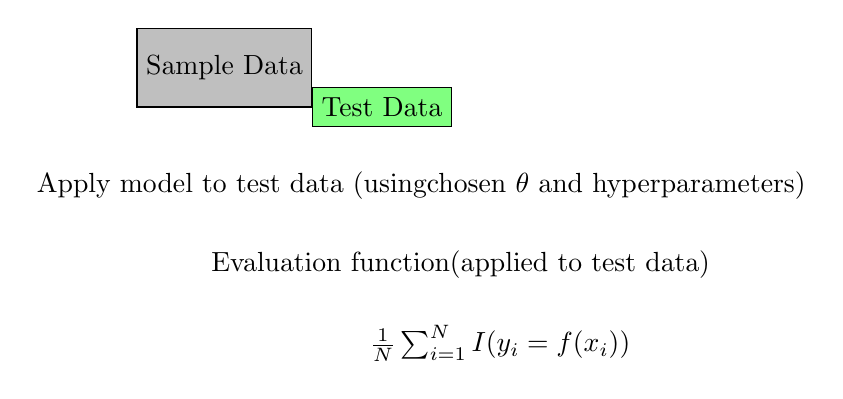
\begin{tikzpicture}
\node[draw, fill=gray!50, minimum width=2cm, minimum height=1cm] (sample) at (0, 0) {Sample Data};
\node[draw, fill=green!50, minimum width=1cm, minimum height=0.5cm] (test) at (2, -0.5) {Test Data};
\node[below of=test, xshift=0.5cm] (apply) {Apply model to test data (using \\ chosen $\theta$ and hyperparameters)};
\node[below of=apply, xshift=0.5cm] (eval) {Evaluation function \\ (applied to test data)};
\node[below of=eval, xshift=0.5cm] (formula) {$\frac{1}{N} \sum_{i=1}^{N} I(y_i = f(x_i))$};
\end{tikzpicture}
%
\subsection{Description}%
This slide, likely from a lecture on Artificial Intelligence Basics, depicts the final stage of the training/test cycle in machine learning.  A large gray rectangle labeled "Sample Data" represents the overall dataset.  A smaller, green rectangle labeled "Test Data" is positioned to the right of the "Sample Data" rectangle, indicating a subset of the data used for testing the trained model.  The text "Apply model to test data (using chosen $\theta$ and hyperparameters)" describes the process of applying the trained model to the test data.  The text "Evaluation function (applied to test data)" describes the process of evaluating the model's performance on the test data.  The formula $\frac{1}{N} \sum_{i=1}^{N} I(y_i = f(x_i))$ is shown below the evaluation function description. This formula represents the calculation of the accuracy of the model on the test data, where $N$ is the number of data points, $y_i$ is the true label for the $i$-th data point, $f(x_i)$ is the predicted label for the $i$-th data point, and $I(y_i = f(x_i))$ is an indicator function that is 1 if the predicted label matches the true label and 0 otherwise. The visual layout emphasizes the final step of evaluating a trained model's performance on unseen test data. The context of the course suggests that this slide is part of a section on model evaluation and testing, specifically focusing on the calculation of accuracy metrics.%
\subsection{Figures}%
\begin{figure}[H]%
\centering%
\begin{subfigure}[b]{0.15\textwidth}%
\centering%

\includegraphics[width=\textwidth]{/Users/ashoksaravanan/Coding/ScribeLec/server/output/CS 243/lectures/10L1-CrossValidation/figures/11.1.png}%
\caption{}%
\end{subfigure}%
\end{figure}

%
\newpage%
\section{Slide 12}%
\label{sec:Slide12}%
\subsection{Content}%
%
\subsection{Description}%
This slide, from a lecture on Artificial Intelligence Basics, outlines the process for diagnosing overfitting in machine learning models.  It visually depicts the comparison of model performance on training and test data.  A gray rectangle labeled "Sample Data" represents the overall dataset.  A teal rectangle labeled "Training Data" and a green rectangle labeled "Test Data" are subsets of the sample data.  The slide emphasizes the crucial step of applying the trained model to both the training and test data.  The text "Apply model to training data (using chosen $\theta$ and hyperparameters)" describes the process of applying the model to the training data using the estimated parameters ($\theta$) and hyperparameters.  Similarly, "Apply model to test data (using chosen $\theta$ and hyperparameters)" describes the application of the model to the test data.  The slide then shows the evaluation function applied to both datasets.  The formula $\frac{1}{N} \sum_{i=1}^{N} I(y_i = f(x_i))$ is used to calculate the accuracy of the model on both the training and test data.  Here, $N$ is the number of data points, $y_i$ is the true label for the $i$-th data point, $f(x_i)$ is the predicted label for the $i$-th data point, and $I(y_i = f(x_i))$ is an indicator function that is 1 if the predicted label matches the true label and 0 otherwise.  The arrows visually connect the application of the model to the evaluation of the model's performance on each dataset.  The context of the course suggests that this slide is part of a section on model evaluation and overfitting detection, focusing on the importance of evaluating model performance on unseen test data to identify overfitting.%
\subsection{Figures}%
\begin{figure}[H]%
\centering%
\begin{subfigure}[b]{0.15\textwidth}%
\centering%

\includegraphics[width=\textwidth]{/Users/ashoksaravanan/Coding/ScribeLec/server/output/CS 243/lectures/10L1-CrossValidation/figures/12.1.png}%
\caption{}%
\end{subfigure}%
\hspace{0.05\textwidth}%
\begin{subfigure}[b]{0.15\textwidth}%
\centering%

\includegraphics[width=\textwidth]{/Users/ashoksaravanan/Coding/ScribeLec/server/output/CS 243/lectures/10L1-CrossValidation/figures/12.2.png}%
\caption{}%
\end{subfigure}%
\end{figure}

%
\newpage%
\section{Slide 13}%
\label{sec:Slide13}%
\subsection{Content}%
%
\subsection{Description}%
This slide, likely from a lecture on Artificial Intelligence Basics, displays a graph illustrating the relationship between model complexity and prediction error for both training and test samples.  The x-axis represents "Model Complexity," ranging from low to high. The y-axis represents "Prediction Error."  Two curves are plotted: one in cyan, representing the prediction error for the training sample, and one in red, representing the prediction error for the test sample.  Both curves are U-shaped, demonstrating a trade-off between model complexity and prediction error.  The training error curve decreases as model complexity increases, reaching a minimum, and then increases again. The test error curve, however, initially decreases, reaches a minimum at a lower complexity than the training error, and then increases more steeply.  The graph visually highlights the concept of overfitting:  a model that is too complex (high complexity) will perform very well on the training data but poorly on unseen test data.  The graph also shows the concept of underfitting: a model that is too simple (low complexity) will perform poorly on both training and test data.  The dashed lines indicate the scenarios of "High Bias, Low Variance" and "Low Bias, High Variance," respectively, providing context for interpreting the graph.  The context of the course suggests that this slide is part of a section on model selection and overfitting, emphasizing the importance of finding the optimal model complexity to minimize both training and test errors.%
\subsection{Figures}%
\begin{figure}[H]%
\centering%
\begin{subfigure}[b]{0.15\textwidth}%
\centering%

\includegraphics[width=\textwidth]{/Users/ashoksaravanan/Coding/ScribeLec/server/output/CS 243/lectures/10L1-CrossValidation/figures/13.1.png}%
\caption{}%
\end{subfigure}%
\end{figure}

%
\newpage%
\section{Slide 14}%
\label{sec:Slide14}%
\subsection{Content}%
%
\subsection{Description}%
This slide, likely from a lecture on Artificial Intelligence Basics, presents the topic of "Hyper-Parameter Tuning."  The title is displayed prominently at the top of the slide.  The content of the slide consists of a simple cartoon image of a small, robotic mail sorter.  The robot has an articulated arm that is in the process of manipulating an object.  The image is stylized and hand-drawn, with a light, whimsical aesthetic.  The text "TWEAK-O-MATIC 9000" is visible in the image, suggesting a humorous or playful approach to the topic of hyper-parameter tuning.  The context of the course suggests that this slide introduces the concept of hyper-parameter tuning as a crucial step in the machine learning process, likely preceding a discussion of methods and techniques for performing this tuning.%
\subsection{Figures}%
\begin{figure}[H]%
\centering%
\begin{subfigure}[b]{0.15\textwidth}%
\centering%

\includegraphics[width=\textwidth]{/Users/ashoksaravanan/Coding/ScribeLec/server/output/CS 243/lectures/10L1-CrossValidation/figures/14.1.png}%
\caption{}%
\end{subfigure}%
\end{figure}

%
\newpage%
\section{Slide 15}%
\label{sec:Slide15}%
\subsection{Content}%
%
\subsection{Description}%
This slide from an Artificial Intelligence Basics lecture demonstrates the concept of overfitting in polynomial curve fitting.  Three graphs are shown, each plotting a cubic function (in green) fitted to the same set of data points (blue circles).  The data points appear to be sampled from a sinusoidal function.  The graphs differ in the degree (M) of the polynomial used to fit the data.

* **M = 1:** The fitted polynomial (red) is a straight line, significantly underfitting the data.  It does not capture the oscillations in the data.

* **M = 3:** The fitted polynomial (red) is a curve that better approximates the data's general shape, but still shows some deviation from the data points.

* **M = 9:** The fitted polynomial (red) closely follows the data points, almost perfectly matching them.  However, this high-degree polynomial exhibits significant oscillations and fluctuations, which are not present in the underlying data. This is a clear example of overfitting. The model is overly complex, fitting the noise in the training data rather than the underlying trend.  The graph visually illustrates how increasing the polynomial degree can lead to a better fit on the training data but a worse fit on unseen data. The context of the course suggests that this slide is part of a section on model complexity, overfitting, and the importance of choosing an appropriate model complexity to avoid overfitting.%
\subsection{Figures}%
\begin{figure}[H]%
\centering%
\begin{subfigure}[b]{0.15\textwidth}%
\centering%

\includegraphics[width=\textwidth]{/Users/ashoksaravanan/Coding/ScribeLec/server/output/CS 243/lectures/10L1-CrossValidation/figures/15.1.png}%
\caption{}%
\end{subfigure}%
\hspace{0.05\textwidth}%
\begin{subfigure}[b]{0.15\textwidth}%
\centering%

\includegraphics[width=\textwidth]{/Users/ashoksaravanan/Coding/ScribeLec/server/output/CS 243/lectures/10L1-CrossValidation/figures/15.2.png}%
\caption{}%
\end{subfigure}%
\hspace{0.05\textwidth}%
\begin{subfigure}[b]{0.15\textwidth}%
\centering%

\includegraphics[width=\textwidth]{/Users/ashoksaravanan/Coding/ScribeLec/server/output/CS 243/lectures/10L1-CrossValidation/figures/15.3.png}%
\caption{}%
\end{subfigure}%
\end{figure}

%
\newpage%
\section{Slide 16}%
\label{sec:Slide16}%
\subsection{Content}%
%
\subsection{Description}%
This slide, from a lecture on Artificial Intelligence Basics, discusses controlling model complexity in polynomial fitting.  The table shows the coefficients ($w_0$, $w_1$, etc.) of polynomial models of different degrees ($M=0, 1, 3, 9$).  The coefficients are presented in a tabular format, with each row representing a coefficient and each column representing a different model degree.  The values in the table represent the coefficients of the polynomial.  The slide highlights that the degree of the polynomial ($M$) directly controls the model's complexity.  The slide prompts the question of how to control complexity when the degree is fixed.  The final statement, "Intuitively, large weights $\rightarrow$ complex model," suggests that the magnitude of the coefficients is related to the complexity of the model.  The context of the course suggests that this slide is part of a discussion on model selection and overfitting, emphasizing the trade-off between model complexity and performance.%
\subsection{Figures}%
\begin{figure}[H]%
\centering%
\begin{subfigure}[b]{0.15\textwidth}%
\centering%

\includegraphics[width=\textwidth]{/Users/ashoksaravanan/Coding/ScribeLec/server/output/CS 243/lectures/10L1-CrossValidation/figures/16.1.png}%
\caption{}%
\end{subfigure}%
\end{figure}

%
\newpage%
\section{Slide 17}%
\label{sec:Slide17}%
\subsection{Content}%

\textbf{Regularized Linear Regression}

New loss function for linear regression:

$E(w) = RSS(w) + \lambda R(w)$

$R(w) = \frac{1}{2} \sum_{i=1}^{k} w_i^2 = w_1^2 + w_2^2 + \dots + w_k^2$, often called a regularizer

$R(w) = \sum_{i=1}^{k} |w_i| = |w_1| + |w_2| + \dots + |w_k|$ also used (called LASSO)

$\lambda$, often called a regularization coefficient

$\bullet$ $\lambda = 0$, no regularization
$\bullet$ $\lambda = +\infty$, best $w$ is 0.
$\bullet$ $\lambda$ controls the trade-off between training error and complexity.
%
\subsection{Description}%
This slide introduces the concept of regularized linear regression.  It defines a new loss function $E(w)$ as the sum of the residual sum of squares (RSS) and a regularization term $R(w)$.  Two types of regularization terms are presented:

* $R(w) = \frac{1}{2} \sum_{i=1}^{k} w_i^2$:  This is the $L_2$ norm (or squared Euclidean norm) of the weight vector $w$, often called ridge regression or L2 regularization.

* $R(w) = \sum_{i=1}^{k} |w_i|$: This is the $L_1$ norm (or Manhattan distance) of the weight vector $w$, often called LASSO (Least Absolute Shrinkage and Selection Operator).

The parameter $\lambda$ is a regularization coefficient that controls the strength of the regularization.  A larger $\lambda$ value increases the importance of the regularization term, potentially leading to a simpler model with smaller weights.  Conversely, a smaller $\lambda$ value gives more weight to the RSS term, potentially leading to a more complex model with larger weights.  The slide highlights that $\lambda = 0$ corresponds to no regularization, while $\lambda = +\infty$ leads to the optimal solution being a model with all weights set to zero.  The final point emphasizes that $\lambda$ controls the trade-off between the training error (measured by RSS) and the complexity of the model (measured by the regularization term).  The context of the course (Artificial Intelligence Basics) suggests that this slide is part of a discussion on model selection and overfitting in linear regression models.%
\subsection{Figures}%
\begin{figure}[H]%
\centering%
\end{figure}

%
\newpage%
\section{Slide 18}%
\label{sec:Slide18}%
\subsection{Content}%

\textbf{Hyperparameter Tuning for Neural Networks}

\textbf{What can be tuned?}

\begin{itemize}
    \item Input: $28 \times 28 \times 1$
    \item Conv: $5 \times 5$, 32 filters, Padding: 2, Pool: $2 \times 2$, stride: 2
    \item $28 \times 28 \times 32$
    \item $14 \times 14 \times 32$
    \item Conv: $5 \times 5$, 64 filters, Padding: 2, Pool: $2 \times 2$, stride: 2
    \item $14 \times 14 \times 64$
    \item Flatten features $\rightarrow$ $1 \times 1 \times 1024$
    \item $7 \times 7 \times 64$
    \item Dropout 0.5
    \item Fc 1.2, 1024
    \item Output: $1 \times 1 \times 10$
\end{itemize}
%
\subsection{Description}%
This slide, from an Artificial Intelligence Basics lecture, displays a diagram of a Convolutional Neural Network (CNN).  It's focused on hyperparameter tuning, showing the different layers and their associated dimensions.  The diagram visually represents the flow of data through the network, from the input layer ($28 \times 28 \times 1$) to the output layer ($1 \times 1 \times 10$).  Each layer is labeled with its type (Input, Conv, Pool, Flatten, Dropout, Fully Connected (FC)), and the dimensions of the data at each stage are shown.  For example, the input is a 28x28 image with one channel.  The first convolutional layer uses 5x5 filters, 32 filters in total, padding of 2, and 2x2 pooling with a stride of 2.  The second convolutional layer uses 5x5 filters, 64 filters in total, padding of 2, and 2x2 pooling with a stride of 2.  The flattened layer transforms the data into a 1x1x1024 format.  The final layer is a fully connected layer with 1024 neurons, followed by a dropout layer with a rate of 0.5, and finally an output layer with 10 neurons.  The slide highlights the various hyperparameters that can be tuned in the network, such as the number of filters, filter size, padding, pooling stride, and dropout rate, to optimize the model's performance.  The context of the course suggests that this slide is part of a section on deep learning architectures and hyperparameter optimization.%
\subsection{Figures}%
\begin{figure}[H]%
\centering%
\begin{subfigure}[b]{0.15\textwidth}%
\centering%

\includegraphics[width=\textwidth]{/Users/ashoksaravanan/Coding/ScribeLec/server/output/CS 243/lectures/10L1-CrossValidation/figures/18.1.png}%
\caption{}%
\end{subfigure}%
\end{figure}

%
\newpage%
\section{Slide 19}%
\label{sec:Slide19}%
\subsection{Content}%

\textbf{Tuning on Held-Out Validation Data}

Now we've got two kinds of unknowns
\begin{itemize}
    \item Parameters: the probabilities $P(X|Y)$, $P(Y)$
    \item Hyperparameters:
    e.g., the amount / type of smoothing to do: $k$, $\alpha$
\end{itemize}

What should we learn where?
\begin{itemize}
    \item Learn parameters from training data
    \item Tune hyperparameters on (different) validation data.
\end{itemize}

Why?
\begin{itemize}
    \item For each value of the hyperparameters, estimate model on training data and test on the held-out validation data
    \item Choose the best values and do a final test on the test data
\end{itemize}

\begin{figure}
\centering
\includegraphics[width=0.5\textwidth]{held_out_validation_graph.png} % Replace with actual image path
\caption{Accuracy vs. k}
\end{figure}
%
\subsection{Description}%
This slide discusses hyperparameter tuning in the context of a machine learning model, likely in an Artificial Intelligence Basics course.  It introduces the concept of "held-out validation data" as a crucial step in model selection.  The slide explains that there are two types of unknowns in a model: parameters and hyperparameters.  Parameters, like probabilities $P(X|Y)$ and $P(Y)$, are learned from the training data.  Hyperparameters, such as the smoothing parameter $k$ or $\alpha$, control the model's behavior and are not directly learned from the data.  The slide emphasizes the importance of tuning hyperparameters on a separate validation dataset.  The process involves evaluating the model's performance on the validation data for different hyperparameter values.  The best hyperparameter values are then selected, and a final evaluation is performed on a separate test dataset to assess the model's generalization ability.  A graph (likely showing accuracy vs. a hyperparameter like $k$) is included, visually demonstrating how the model's performance varies with different hyperparameter settings.  The context of the course suggests that this slide is part of a discussion on model evaluation and selection techniques.%
\subsection{Figures}%
\begin{figure}[H]%
\centering%
\begin{subfigure}[b]{0.15\textwidth}%
\centering%

\includegraphics[width=\textwidth]{/Users/ashoksaravanan/Coding/ScribeLec/server/output/CS 243/lectures/10L1-CrossValidation/figures/19.1.png}%
\caption{}%
\end{subfigure}%
\hspace{0.05\textwidth}%
\begin{subfigure}[b]{0.15\textwidth}%
\centering%

\includegraphics[width=\textwidth]{/Users/ashoksaravanan/Coding/ScribeLec/server/output/CS 243/lectures/10L1-CrossValidation/figures/19.2.png}%
\caption{}%
\end{subfigure}%
\hspace{0.05\textwidth}%
\begin{subfigure}[b]{0.15\textwidth}%
\centering%

\includegraphics[width=\textwidth]{/Users/ashoksaravanan/Coding/ScribeLec/server/output/CS 243/lectures/10L1-CrossValidation/figures/19.3.png}%
\caption{}%
\end{subfigure}%
\end{figure}

%
\newpage%
\section{Slide 20}%
\label{sec:Slide20}%
\subsection{Content}%

\textbf{Learning curves illuminate likely causes of error}

\begin{figure}
\centering
\includegraphics[width=0.5\textwidth]{learning_curve.png} % Replace with actual image path
\caption{Learning Curve}
\end{figure}

\textbf{Accuracy} \\
\textbf{Model complexity} \\
\textbf{Training set} \\
\textbf{Test set}
%
\subsection{Description}%
This slide, from an Artificial Intelligence Basics lecture, introduces the concept of learning curves.  It states that learning curves help identify potential sources of error in a machine learning model.  The slide displays a simple graph, likely a plot of accuracy versus model complexity.  Two curves are shown: one representing the accuracy on the training set and the other representing the accuracy on a separate test set.  The x-axis likely represents the model complexity (e.g., number of parameters, depth of a neural network).  The y-axis represents the accuracy of the model.  The graph visually depicts how the accuracy of the model changes as the model complexity increases.  The labels "Training set" and "Test set" indicate that the curves correspond to the model's performance on the training data and a separate, unseen test data set.  The context of the course suggests that this slide is part of a discussion on model evaluation and overfitting, where learning curves are used to diagnose issues like high bias or high variance.%
\subsection{Figures}%
\begin{figure}[H]%
\centering%
\begin{subfigure}[b]{0.15\textwidth}%
\centering%

\includegraphics[width=\textwidth]{/Users/ashoksaravanan/Coding/ScribeLec/server/output/CS 243/lectures/10L1-CrossValidation/figures/20.1.png}%
\caption{}%
\end{subfigure}%
\end{figure}

%
\newpage%
\section{Slide 21}%
\label{sec:Slide21}%
\subsection{Content}%
%
\subsection{Description}%
This slide, from an Artificial Intelligence Basics course, discusses the decision of whether to acquire more data or modify the model when dealing with underfitting.  It presents a graph (learning curve) depicting the relationship between model complexity (likely on the x-axis) and accuracy (likely on the y-axis).  Two curves are shown: one for the training set and one for the test set.  The graph shows an underfitting scenario, where both the training and test set accuracies are low and relatively flat, indicating that the model is not learning the underlying patterns in the data.  The text below the graph states that if the learning curves continue to increase (as model complexity increases), then adding more data will not significantly improve the model's performance.  In this case, the solution is to increase the complexity of the model, rather than collecting more data.  The context of the slide suggests a discussion on model selection and the trade-off between data and model complexity in machine learning.%
\subsection{Figures}%
\begin{figure}[H]%
\centering%
\begin{subfigure}[b]{0.15\textwidth}%
\centering%

\includegraphics[width=\textwidth]{/Users/ashoksaravanan/Coding/ScribeLec/server/output/CS 243/lectures/10L1-CrossValidation/figures/21.1.png}%
\caption{}%
\end{subfigure}%
\end{figure}

%
\newpage%
\section{Slide 22}%
\label{sec:Slide22}%
\subsection{Content}%
%
\subsection{Description}%
This slide, from an Artificial Intelligence Basics course, discusses the decision of whether to acquire more data or modify the model when dealing with overfitting.  It presents a graph (learning curve) depicting the relationship between model complexity (likely on the x-axis, though not explicitly shown) and accuracy (likely on the y-axis).  Two curves are shown: one for the training set and one for the test set.  The graph shows an overfitting scenario, where the training set accuracy is high, but the test set accuracy is lower and starts to decrease as the model complexity increases.  This indicates that the model is learning the training data too well, including noise and irrelevant details, and is not generalizing well to unseen data.  The text below the graph states that if the test set accuracy starts to decrease, it suggests the model is overfitting.  In this case, the solution is to either get more data to better represent the underlying patterns or to regularize the model during learning to reduce its complexity and prevent it from focusing too much on the idiosyncrasies of the training data. The context of the slide suggests a discussion on model selection and the trade-off between data and model complexity in machine learning, specifically addressing the issue of overfitting.%
\subsection{Figures}%
\begin{figure}[H]%
\centering%
\begin{subfigure}[b]{0.15\textwidth}%
\centering%

\includegraphics[width=\textwidth]{/Users/ashoksaravanan/Coding/ScribeLec/server/output/CS 243/lectures/10L1-CrossValidation/figures/22.1.png}%
\caption{}%
\end{subfigure}%
\end{figure}

%
\newpage%
\section{Slide 23}%
\label{sec:Slide23}%
\subsection{Content}%

\textbf{When to get more data vs. use different model}

\begin{figure}
\centering
\includegraphics[width=0.3\textwidth]{learning_curve.png} % Replace with actual image path
\caption{Learning Curve}
\end{figure}

\textbf{Just right} \\
\textbf{Training set} \\
\textbf{Test set} \\

If learning curve on training data reaches a high plateau and test performance is similar \\
$\implies$ stop to celebrate, this almost never happens!
%
\subsection{Description}%
This slide, from an Artificial Intelligence Basics lecture, discusses the decision of whether to acquire more data or modify the model when evaluating a machine learning model.  It presents a graph (learning curve) depicting the relationship between model complexity (likely on the x-axis, though not explicitly shown) and accuracy (likely on the y-axis).  Two curves are shown: one for the training set and one for the test set.  The graph shows a scenario where the training set accuracy reaches a high plateau, and the test set accuracy is similar.  The text below the graph states that if the learning curve on the training data reaches a high plateau and the test performance is similar, then it's a sign that the model is performing well and the model complexity is appropriate.  The text further emphasizes that this scenario is rare, implying that in most cases, further improvements are possible by either acquiring more data or modifying the model. The context of the slide suggests a discussion on model selection and the trade-off between data and model complexity in machine learning, specifically addressing the point where the model is performing well on both training and test data.%
\subsection{Figures}%
\begin{figure}[H]%
\centering%
\begin{subfigure}[b]{0.15\textwidth}%
\centering%

\includegraphics[width=\textwidth]{/Users/ashoksaravanan/Coding/ScribeLec/server/output/CS 243/lectures/10L1-CrossValidation/figures/23.1.png}%
\caption{}%
\end{subfigure}%
\end{figure}

%
\newpage%
\section{Slide 24}%
\label{sec:Slide24}%
\subsection{Content}%
%
\subsection{Description}%
This slide, from an Artificial Intelligence Basics course, presents a visual aid to help students understand when to acquire more data versus modifying the model in machine learning.  It's divided into three sections: Underfitting, Overfitting, and Just Right.

* **Underfitting:**  A graph shows a learning curve where both the training and test set accuracies are low and relatively flat, indicating that the model is not learning the underlying patterns in the data.  The solution is to increase the complexity of the model.

* **Overfitting:** A graph shows a learning curve where the training set accuracy is high, but the test set accuracy is lower and starts to decrease as the model complexity increases. This indicates that the model is learning the training data too well, including noise and irrelevant details, and is not generalizing well to unseen data. The solution is to get more data and/or regularize the model during learning.

* **Just Right:** A graph shows a learning curve where the training set accuracy reaches a high plateau, and the test set accuracy is similar. This indicates that the model is performing well and the model complexity is appropriate.  The text emphasizes that this scenario is rare.

The slide uses graphs (learning curves) to illustrate the relationship between model complexity and accuracy for training and test sets in each scenario.  The text below each graph provides guidance on the appropriate action to take (increase model complexity, get more data, or regularize). The context of the course is machine learning model selection and the trade-off between data and model complexity.  The slide is designed to help students understand the different scenarios and make informed decisions about data acquisition and model modification.%
\subsection{Figures}%
\begin{figure}[H]%
\centering%
\begin{subfigure}[b]{0.15\textwidth}%
\centering%

\includegraphics[width=\textwidth]{/Users/ashoksaravanan/Coding/ScribeLec/server/output/CS 243/lectures/10L1-CrossValidation/figures/24.1.png}%
\caption{}%
\end{subfigure}%
\hspace{0.05\textwidth}%
\begin{subfigure}[b]{0.15\textwidth}%
\centering%

\includegraphics[width=\textwidth]{/Users/ashoksaravanan/Coding/ScribeLec/server/output/CS 243/lectures/10L1-CrossValidation/figures/24.2.png}%
\caption{}%
\end{subfigure}%
\hspace{0.05\textwidth}%
\begin{subfigure}[b]{0.15\textwidth}%
\centering%

\includegraphics[width=\textwidth]{/Users/ashoksaravanan/Coding/ScribeLec/server/output/CS 243/lectures/10L1-CrossValidation/figures/24.3.png}%
\caption{}%
\end{subfigure}%
\end{figure}

%
\newpage%
\section{Slide 25}%
\label{sec:Slide25}%
\subsection{Content}%
%
\subsection{Description}%
This slide describes the process of S-fold cross-validation, a technique used in machine learning to evaluate a model's performance.  The method is presented in the context of an Artificial Intelligence Basics course.  The slide visually depicts a 5-fold cross-validation example, where the data is divided into 5 equal parts.  Each part is used as a validation set once, while the remaining parts are used as the training set.  This process is repeated 5 times, resulting in 5 different training and validation sets.  The slide emphasizes that every data point is used as a validation point exactly once.  The text also explains the steps involved: splitting the training data into S equal parts, using each part as a validation set, choosing the hyper-parameter that yields the best average performance across all runs, and the specific case of leave-one-out cross-validation.  The visual representation uses white boxes for training data and red boxes for validation data, making the process clear and easy to understand.  The context of the slide is model evaluation and hyperparameter tuning in machine learning.%
\subsection{Figures}%
\begin{figure}[H]%
\centering%
\begin{subfigure}[b]{0.15\textwidth}%
\centering%

\includegraphics[width=\textwidth]{/Users/ashoksaravanan/Coding/ScribeLec/server/output/CS 243/lectures/10L1-CrossValidation/figures/25.1.png}%
\caption{}%
\end{subfigure}%
\end{figure}

%
\newpage%
\section{Slide 26}%
\label{sec:Slide26}%
\subsection{Content}%
%
\subsection{Description}%
This slide, from an Artificial Intelligence Basics lecture, presents a visual representation of the data analysis pipeline.  It's a flowchart-like diagram showing the sequential steps involved in a typical machine learning project.  The four main stages are: Collect Data, Design Model, Infer Parameters, and Apply Model.  Each stage has a brief description of potential issues or challenges that can arise at each step.  For example, the "Collect Data" stage notes that the data might contain unexpected errors or outliers.  The "Design Model" stage highlights that the model's assumptions might not perfectly match the data's characteristics.  The "Infer Parameters" stage points out that algorithm code can have bugs or errors, especially due to approximations.  Finally, the "Apply Model" stage emphasizes that the test data might differ significantly from the training data, potentially leading to poor generalization.  The slide is designed to illustrate the iterative and potentially problematic nature of the data analysis process, emphasizing the importance of careful consideration at each step.%
\subsection{Figures}%
\begin{figure}[H]%
\centering%
\begin{subfigure}[b]{0.15\textwidth}%
\centering%

\includegraphics[width=\textwidth]{/Users/ashoksaravanan/Coding/ScribeLec/server/output/CS 243/lectures/10L1-CrossValidation/figures/26.1.png}%
\caption{}%
\end{subfigure}%
\hspace{0.05\textwidth}%
\begin{subfigure}[b]{0.15\textwidth}%
\centering%

\includegraphics[width=\textwidth]{/Users/ashoksaravanan/Coding/ScribeLec/server/output/CS 243/lectures/10L1-CrossValidation/figures/26.10.png}%
\caption{}%
\end{subfigure}%
\hspace{0.05\textwidth}%
\begin{subfigure}[b]{0.15\textwidth}%
\centering%

\includegraphics[width=\textwidth]{/Users/ashoksaravanan/Coding/ScribeLec/server/output/CS 243/lectures/10L1-CrossValidation/figures/26.11.png}%
\caption{}%
\end{subfigure}%
\hspace{0.05\textwidth}%
\begin{subfigure}[b]{0.15\textwidth}%
\centering%

\includegraphics[width=\textwidth]{/Users/ashoksaravanan/Coding/ScribeLec/server/output/CS 243/lectures/10L1-CrossValidation/figures/26.12.png}%
\caption{}%
\end{subfigure}%
\hspace{0.05\textwidth}%
\begin{subfigure}[b]{0.15\textwidth}%
\centering%

\includegraphics[width=\textwidth]{/Users/ashoksaravanan/Coding/ScribeLec/server/output/CS 243/lectures/10L1-CrossValidation/figures/26.13.png}%
\caption{}%
\end{subfigure}%
\end{figure}

%
\newpage%
\section{Slide 27}%
\label{sec:Slide27}%
\subsection{Content}%
%
\subsection{Description}%
This slide, from an Artificial Intelligence Basics course, displays a graph illustrating the relationship between model complexity and prediction error for both training and test samples.  The x-axis represents the model complexity, ranging from low to high. The y-axis represents the prediction error.  Two curves are plotted: one in red for the training sample and one in cyan for the test sample.

The red curve (training sample) shows a U-shaped relationship, decreasing rapidly at first as model complexity increases, reaching a minimum, and then increasing again.  The cyan curve (test sample) also shows a U-shaped relationship, but it has a minimum at a higher complexity than the training sample curve.  The minimum point of the test sample curve is higher than the minimum point of the training sample curve.

The graph visually demonstrates the concept of bias-variance trade-off in machine learning models.  The labels "High Bias, Low Variance" and "Low Bias, High Variance" are placed on the graph to indicate the different scenarios.  The graph suggests that there is an optimal model complexity that minimizes the prediction error on both the training and test sets.  The context of the slide is model selection and the trade-off between model complexity and generalization performance in machine learning.%
\subsection{Figures}%
\begin{figure}[H]%
\centering%
\begin{subfigure}[b]{0.15\textwidth}%
\centering%

\includegraphics[width=\textwidth]{/Users/ashoksaravanan/Coding/ScribeLec/server/output/CS 243/lectures/10L1-CrossValidation/figures/27.1.png}%
\caption{}%
\end{subfigure}%
\end{figure}

%
\newpage%
\end{document}